% External-choice merge: two receives from the SAME sender O, with distinct labels,
% combine into one Branch offering both — the rule that makes a bystander projectable.
% Palette: recv=sky, branch=sky-deep, merge-op=teal.
\documentclass[border=10pt]{standalone}
\usepackage{tikz}
\usepackage{amssymb}
\usepackage{xcolor}
\usetikzlibrary{arrows.meta, positioning, fit, backgrounds, calc}
\definecolor{recv}{HTML}{0284C7}
\definecolor{branch}{HTML}{075985}
\definecolor{op}{HTML}{0D9488}
\definecolor{ink}{HTML}{0C4A6E}
\begin{document}
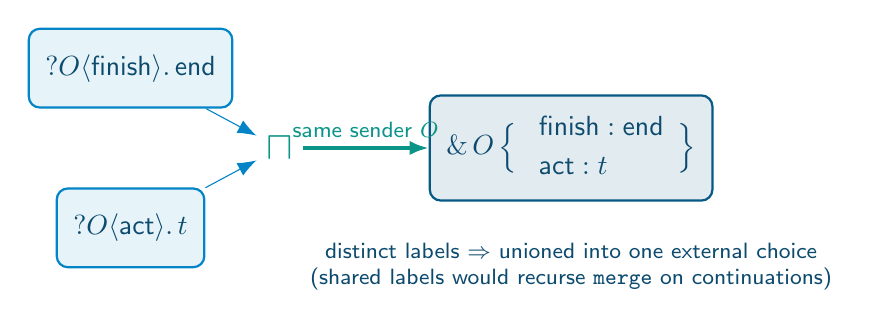
\begin{tikzpicture}[font=\sffamily, >={Latex[length=2.4mm]},
    box/.style={draw, thick, rounded corners, align=center, inner sep=6pt, minimum height=10mm},
    rb/.style={box, draw=recv, fill=recv!10, text=ink},
    bb/.style={box, draw=branch, fill=branch!12, text=ink}]

  \node[rb] (a) {$?O\langle \mathsf{finish}\rangle . \,\mathsf{end}$};
  \node[rb, below=10mm of a] (b) {$?O\langle \mathsf{act}\rangle . \,t$};

  \node[op, font=\sffamily\Large\bfseries, right=16mm of $(a)!0.5!(b)$] (m) {$\sqcap$};

  \node[bb, right=16mm of m] (r)
    {$\&\,O\,\Big\{\;\begin{array}{l}\mathsf{finish} : \mathsf{end}\\[2pt]\mathsf{act} : t\end{array}\Big\}$};

  \draw[->, recv] (a) -- (m);
  \draw[->, recv] (b) -- (m);
  \draw[->, op, very thick] (m) -- node[above, font=\sffamily\footnotesize, text=op]{same sender $O$} (r);

  \node[font=\sffamily\footnotesize, text=ink, below=4mm of r, align=center]
    {distinct labels $\Rightarrow$ unioned into one external choice\\(shared labels would recurse \texttt{merge} on continuations)};
\end{tikzpicture}
\end{document}
